\documentclass[tikz,border=3.14mm]{standalone}
\begin{document}
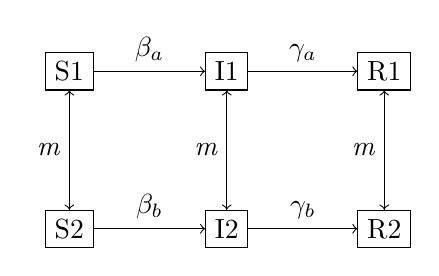
\begin{tikzpicture}
        % Nodes for patch 1
        \node[draw] (S1) at (0,0) {S1};
        \node[draw] (I1) at (2,0) {I1};
        \node[draw] (R1) at (4,0) {R1};
        
        % Nodes for patch 2
        \node[draw] (S2) at (0,-2) {S2};
        \node[draw] (I2) at (2,-2) {I2};
        \node[draw] (R2) at (4,-2) {R2};
        
        \draw[->] (S1) -- node[midway,above] {$\beta_a$} (I1);
        \draw[->] (S2) -- node[midway,above] {$\beta_b$} (I2);

        \draw[->] (I1) -- node[midway,above] {$\gamma_a$} (R1);
        \draw[->] (I2) -- node[midway,above] {$\gamma_b$} (R2);

        % Migration edges
        \draw[->] (S1) -- node[midway, left] {$\textit m$} (S2);
        \draw[->] (S2) -- (S1);
        \draw[->] (I1) -- node[midway, left] {$\textit m$}  (I2);
        \draw[->] (I2) -- (I1);
        \draw[->] (R1) -- node[midway, left] {$\textit m$}  (R2);
        \draw[->] (R2) -- (R1);

\end{tikzpicture}
\end{document}
